% !Mode:: "TeX:UTF-8"

\chapter{}
\textbf{
There's a natural intuition that two nodes that are far apart in a communication network——separated by many hops——have a more tenuous connection than two nodes that are close together. There are a number of algorithmic results that are based to some extent on different ways of making this notion precise. Here's one that involves the susceptibility of paths to the deletion of nodes.
}

\textbf{
Suppose that an $n$-node undirected graph $G=(V,E)$ contains two nodes $s$ and $t$ such that the distance between $s$ and $t$ is strictly greater than $n/2$. Show that there must exist some node $v$, not equal to either $s$ or $t$, such that deleting $v$ from $G$ destroys all $s-t$ paths.(In other words, the graph obtained from $G$ by deleting $v$ contains no path from $s$ to $t$.) Give an algorithm with running time $O(m+n)$ to find such a node $v$.
}

\hspace*{\fill} \\

According to BFS algorithm and the given conditions, as shown in figure~\ref{figure_5_1}, there exists an separated layers satisfying that the count of layers is $m$ and $m-1> n/2 $. The problem is equal to Pigeon nest problem. Notice that there remain at most $n-2$ vertexes which will be put into $m-1$ cells. And notice that $2(m-1)>n>n-2$. So there must be at least one cell(actually two cells) that contains only one vertex. That is to say there exists some node $v$ that satisfying our goal.
\begin{figure}[!htbp]
  \centering
  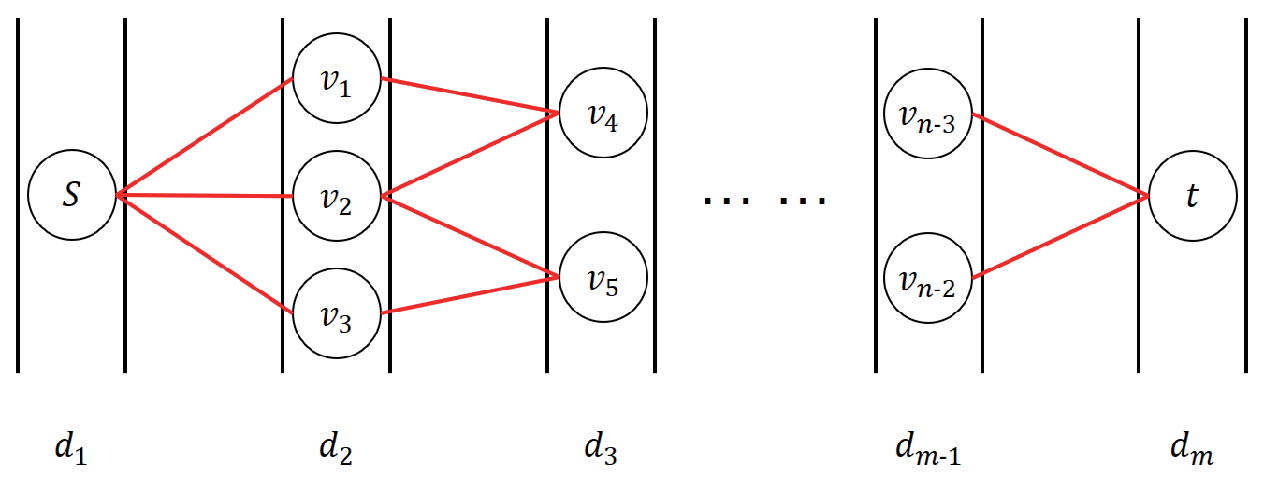
\includegraphics[width=0.7\textwidth]{figures/5_1.eps}\\
  \caption{The layers of breadth-first search}\label{find_key_point}
\end{figure}

We next give an algorithm to find one of these vertex. Generally speaking, we just need to execute depth-first traversal rooted at $S$ and get tree $T$. Because $s$ and $t$ are connected, $t$ is definitely in $T$. Besides, it is sure that there is at leat one layer that contains one vertex. So we just need to find this vertex. We give the detail process in Alg~\ref{find_key_point}.

\begin{algorithm}[!htbp]
\caption{The pivotal vertex discovering}
\label{find_key_point}
\begin{algorithmic}[1]
\REQUIRE $s$
\STATE{Set Discovered[$s$]=$true$ and Discovered[$v$]=$false$ for all other $v$}
\STATE{Initialize $L[0]$ to consist of the single element $s$}
\STATE{Set the layer count $i$=0}
\STATE{Set result node rnode = $null$}
\WHILE{$L[i]\neq \phi$}
    \IF{Size($L[i]$) = 1 and $i>0$}
        \STATE{Set rnode = $L[i][0]$}
        \STATE{break}
    \ENDIF
    \STATE{Initialize an empty list L[$i+1$]}
    \FOR{each node $u\in L[i]$}
        \STATE{Consider each edge $(u,v)$ incident to $u$}
        \IF{Discovered[$v$]=$false$}
            \STATE{Set Discovered[$v$]=$true$}
            \STATE{Add $v$ to the list $L[i+1]$}
        \ENDIF
    \ENDFOR
    \STATE{Increment the layer counter $i$ by one}
\ENDWHILE   
\STATE Return rnode
\end{algorithmic}
\end{algorithm}

As showed in Alg~\ref{find_key_point}, we test the number of each layer(line 6). When the count of layer number is one and it is not the first layer, we set the result node as the single element in this layer and break the loop.
